\chapter{Phân loại MedMNIST (ChestMNIST) bằng ANN}

\section{Tổng quan}

Khác với MNIST và FashionMNIST, ChestMNIST là bài toán ảnh y sinh đa nhãn với mức độ khó cao hơn rõ rệt~\cite{yang2022medmnistv2}. Mỗi ảnh X-quang ngực có thể đồng thời mang nhiều bệnh, dữ liệu bị mất cân bằng mạnh, và benchmark chính thức ưu tiên \textit{AUC} cùng \textit{ACC} thay vì chỉ nhìn accuracy theo kiểu một nhãn~\cite{medmnist_site}. Vì vậy, chương này tiếp tục đi theo cùng logic của Chương 1: bắt đầu từ baseline đơn giản nhất để xem raw pixel thuần đi được đến đâu, sau đó lần lượt bổ sung weighted loss, cross-validation và feature engineering phù hợp với ảnh X-quang.

\section{Phát biểu bài toán}

ChestMNIST là bài toán \textit{multi-label classification} trên ảnh X-quang ngực kích thước $28 \times 28$~\cite{yang2022medmnistv2}. Đầu vào của mô hình là ảnh xám $28 \times 28$, tương đương $784$ pixel. Đầu ra của mô hình là vector logits $14$ chiều, trong đó mỗi phần tử trả lời một câu hỏi nhị phân độc lập: nhãn bệnh tương ứng có xuất hiện hay không. Vì mỗi ảnh có thể đồng thời mang nhiều bệnh, đầu ra không dùng softmax mà dùng $14$ xác suất sigmoid độc lập.

Trong chương này có hai cách khai thác split dữ liệu. Baseline naive dùng trực tiếp ba split chính thức train/validation/test của ChestMNIST để lấy mặt bằng ban đầu. Hai biến thể mạnh hơn không tune trực tiếp trên validation chính thức; thay vào đó, chỉ split train được chia tiếp bằng \textit{3-fold multilabel stratified cross-validation}, còn split test chính thức vẫn được giữ riêng cho đánh giá cuối. Cách làm này giúp test tách biệt hoàn toàn khỏi quá trình huấn luyện.

\begin{table}[H]
\centering
\caption{Phát biểu bài toán và thiết lập dữ liệu của ChestMNIST}
\label{tab:chestmnist-problem-setup}
\begin{tabular}{l c}
\toprule
Thành phần & Giá trị \\
\midrule
Kiểu bài toán & Multi-label classification \\
Đầu vào & Ảnh X-quang ngực xám $28 \times 28$ \\
Đầu ra & Vector logits $14$ chiều \\
Số nhãn & $14$ nhãn bệnh độc lập \\
Train chính thức & $78{,}468$ mẫu \\
Validation chính thức & $11{,}219$ mẫu \\
Test chính thức & $22{,}433$ mẫu \\
Thiết lập Lab 03 & Naive dùng train/val/test; các biến thể sau dùng 3-fold CV trên train và test ở cuối \\
\bottomrule
\end{tabular}
\end{table}


\section{Mô hình và tham số}
\subsection{Baseline naive}

Baseline naive là điểm xuất phát để kiểm tra xem ANN thuần trên raw pixel có thể học được bao nhiêu trên ChestMNIST. Ảnh đầu vào được chuẩn hóa về $[0,1]$, trải phẳng thành vector $784$ chiều, rồi đưa qua MLP:
\[
784 \rightarrow 512 \rightarrow 256 \rightarrow 14.
\]
Hai tầng ẩn dùng ReLU; tầng cuối giữ logits thô cho $14$ nhãn bệnh. Cấu hình $784 \rightarrow 512 \rightarrow 256 \rightarrow 14$ được chọn theo tinh thần baseline: đủ nhỏ để đóng vai trò mốc tối thiểu, nhưng vẫn có hai tầng ẩn để ANN có thể tái tổ hợp raw pixel thành biểu diễn phi tuyến cơ bản. Loss được chọn là BCEWithLogitsLoss vì đây là bài toán đa nhãn và mỗi nhãn bệnh phải được tối ưu như một bài toán nhị phân riêng; dùng softmax hoặc cross-entropy một nhãn ở đây sẽ làm sai bản chất bài toán. Baseline này chưa dùng BatchNorm, Dropout, feature engineering hay weighted loss.

\begin{table}[H]
\centering
\caption{Kết quả baseline naive single-branch ANN trên ChestMNIST}
\label{tab:chestmnist-naive-results}
\begin{tabular}{l c}
\toprule
Chỉ số & Giá trị \\
\midrule
Best validation macro AUC & 0.7185 \\
Test ACC & 0.9475 \\
Final validation macro F1 & 0.0063 \\
Test macro AUC & 0.7088 \\
Test macro F1 & 0.0069 \\
Số epoch đã chạy & 45 \\
Kiến trúc mạng & $784 \rightarrow 512 \rightarrow 256 \rightarrow 14$ \\
\bottomrule
\end{tabular}
\end{table}


\begin{figure}[H]
  \centering
  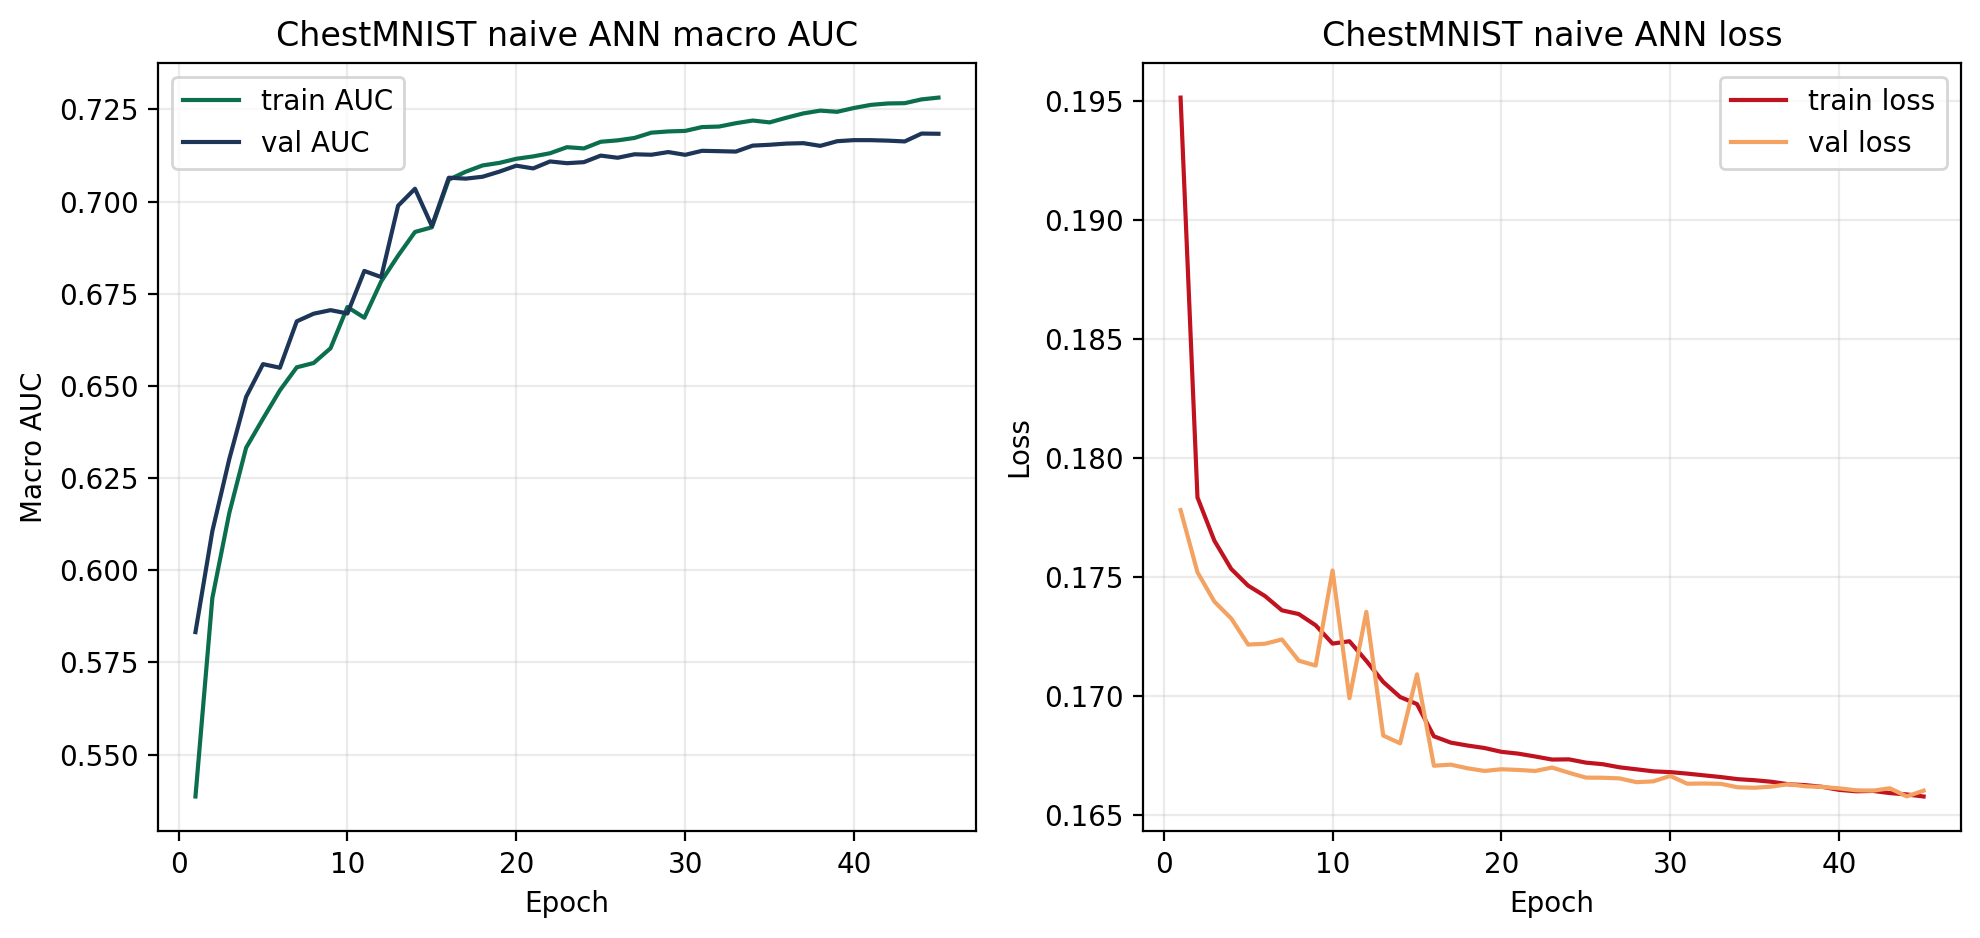
\includegraphics[width=0.95\textwidth]{figures/chestmnist-ann/training_curves.png}
  \caption{Diễn biến macro AUC và loss của baseline naive ANN trên ChestMNIST trong 45 epoch.}
  \label{fig:chestmnist-training-curves}
\end{figure}

\begin{figure}[H]
  \centering
  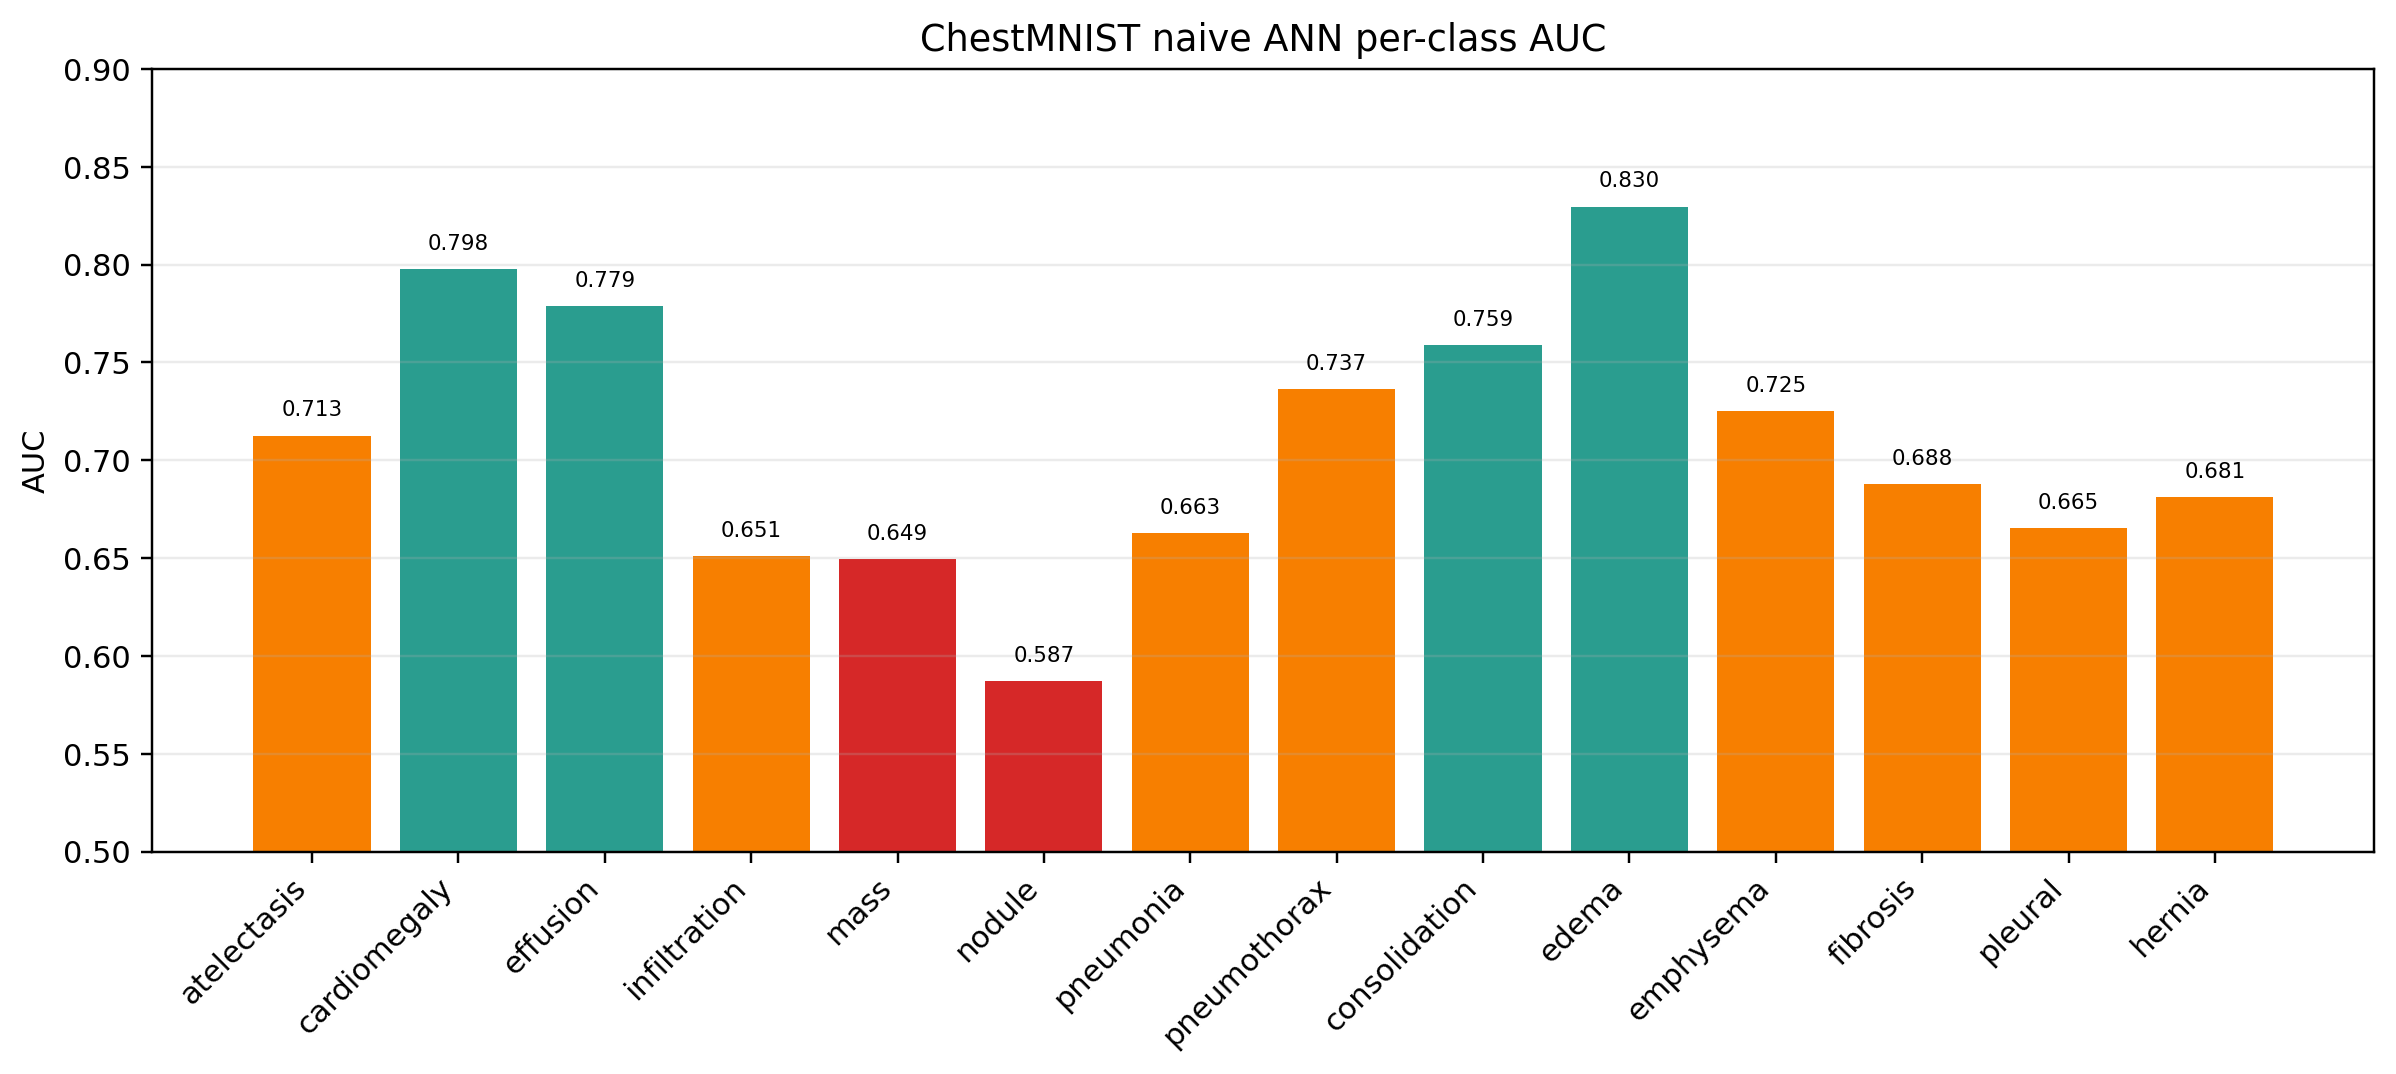
\includegraphics[width=0.95\textwidth]{figures/chestmnist-ann/per_class_auc.png}
  \caption{AUC theo từng nhãn bệnh của baseline naive trên ChestMNIST.}
  \label{fig:chestmnist-per-class-auc}
\end{figure}

\begin{figure}[H]
  \centering
  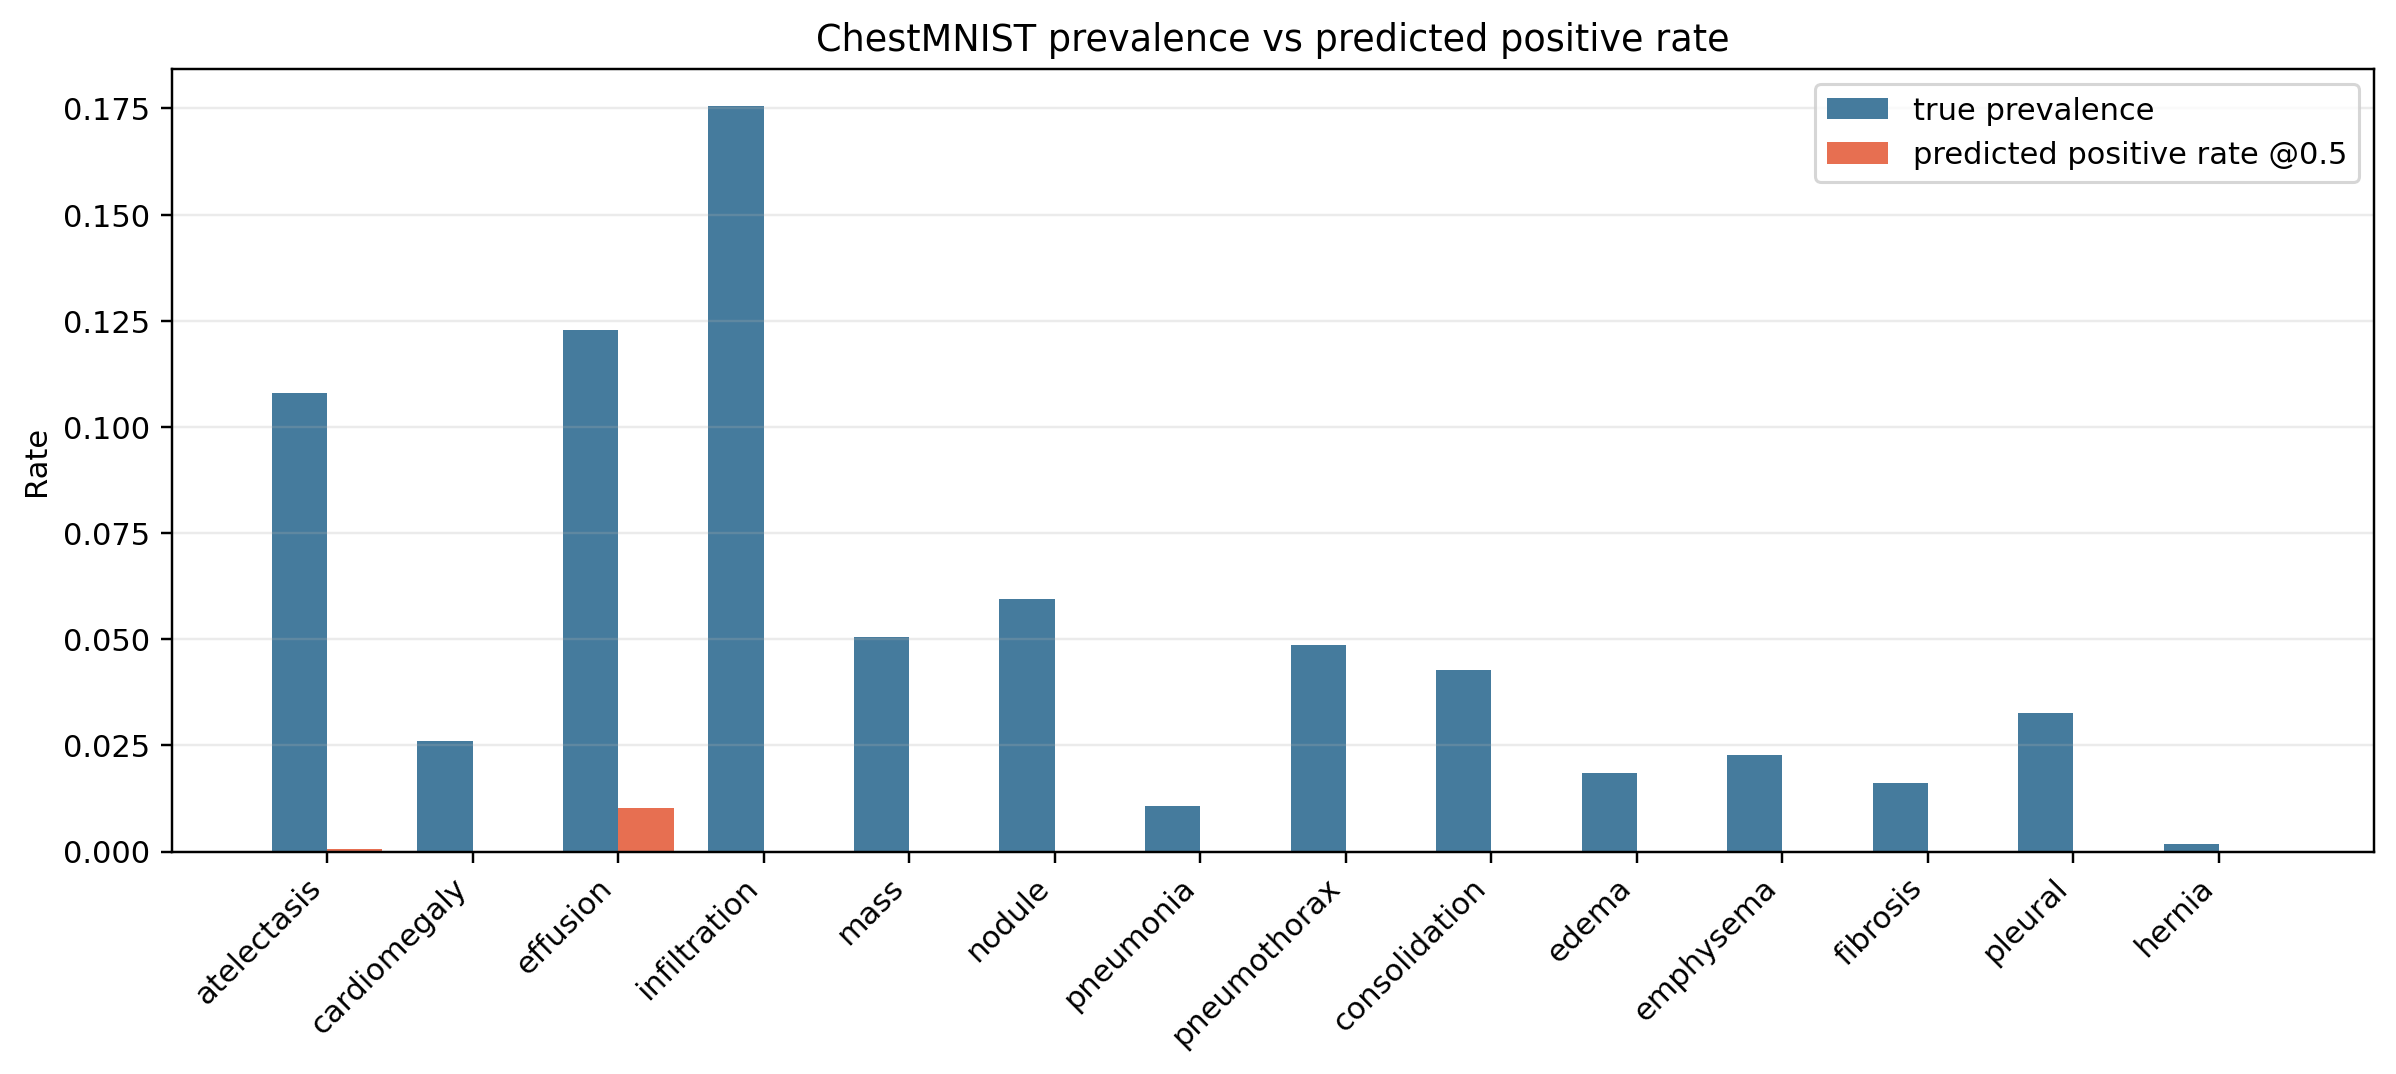
\includegraphics[width=0.95\textwidth]{figures/chestmnist-ann/prevalence_vs_pred_rate.png}
  \caption{So sánh tỷ lệ dương thật và tỷ lệ dương dự đoán ở ngưỡng $0.5$ của baseline naive trên ChestMNIST.}
  \label{fig:chestmnist-prevalence-vs-pred-rate}
\end{figure}

\begin{table}[H]
\centering
\caption{Một số nhãn dễ và khó nhất của baseline naive trên ChestMNIST}
\label{tab:chestmnist-per-class-auc}
\begin{tabular}{l c c c c}
\toprule
Nhãn & AUC & F1 & Tỷ lệ dương thật & Tỷ lệ dương dự đoán \\
\midrule
Edema & 0.8296 & 0.0000 & 0.0184 & 0.0000 \\
Cardiomegaly & 0.7978 & 0.0000 & 0.0259 & 0.0000 \\
Effusion & 0.7787 & 0.0891 & 0.1228 & 0.0103 \\
Nodule & 0.5872 & 0.0000 & 0.0595 & 0.0000 \\
Mass & 0.6494 & 0.0000 & 0.0505 & 0.0000 \\
Infiltration & 0.6508 & 0.0020 & 0.1755 & 0.0002 \\
\bottomrule
\end{tabular}
\end{table}


Baseline naive đạt \textit{test macro AUC} $0.7088$ và \textit{test ACC} $0.9475$. AUC cho thấy mô hình mới chỉ học được tín hiệu phân biệt ở mức vừa phải, trong khi ACC rất cao chủ yếu vì dữ liệu có quá nhiều nhãn âm. Hình prevalence-vs-pred-rate cho thấy mô hình gần như đoán âm cho phần lớn nhãn ở ngưỡng $0.5$, nên ACC cao nhưng chưa phản ánh tốt khả năng phát hiện ca bệnh thật.

Từ kết quả này, có thể thấy vấn đề chính không phải ANN hoàn toàn bất lực trước ảnh X-quang, mà là động lực học huấn luyện hiện tại quá thiên về việc giữ nhãn âm. Vì vậy, bước cải tiến kế tiếp hợp lý nhất là thêm weighted loss và cross-validation để buộc mô hình chú ý nhiều hơn tới ca dương và ổn định hơn qua nhiều fold.

\subsection{Weighted ANN với cross-validation nội bộ}

Kết quả của baseline naive cho thấy hai vấn đề xuất hiện đồng thời. Thứ nhất, raw pixel thuần vẫn chứa tín hiệu phân biệt nhất định, thể hiện qua macro AUC vượt rõ mức ngẫu nhiên; tuy nhiên tín hiệu đó chưa đủ mạnh để đưa mô hình lên gần các benchmark tốt hơn. Thứ hai, mô hình có xu hướng chọn nghiệm an toàn theo hướng giữ nhiều nhãn âm, nên ACC cao nhưng chất lượng tách ca bệnh theo AUC còn hạn chế. Từ insight này, bước cải tiến hợp lý không phải là thêm handcrafted feature ngay lập tức, mà trước hết phải sửa đúng động lực học huấn luyện để mô hình coi trọng nhãn dương hơn và đánh giá nội bộ ổn định hơn trên tập train.

Biến thể thứ hai vì vậy vẫn giữ đầu vào raw pixel để cô lập ảnh hưởng của kỹ thuật huấn luyện, nhưng thay đổi đồng thời cả kiến trúc và protocol. MLP được mở rộng thành:
\[
784 \rightarrow 1024 \rightarrow 512 \rightarrow 256 \rightarrow 14.
\]
Chiều rộng tầng đầu tăng lên $1024$ để ANN có đủ năng lực biểu diễn hơn cho ảnh X-quang, vốn có cấu trúc khó hơn đáng kể so với chữ số viết tay và có nhiều tổn thương chỉ biểu hiện bằng thay đổi texture rất nhẹ. Hai tầng sau giảm dần về $512$ và $256$ để nén dần biểu diễn đã học, tránh giữ kích thước ẩn lớn suốt toàn mạng khiến số tham số tăng nhanh nhưng không bổ sung tương xứng về khả năng tổng quát hóa. BatchNorm được thêm để ổn định phân phối kích hoạt giữa các tầng ẩn, còn Dropout giúp giảm sự phụ thuộc quá mức giữa các neuron trong bối cảnh số nhãn dương tương đối ít. Nói cách khác, phương pháp này không chỉ rộng hơn baseline, mà còn được tổ chức theo hướng “mở rộng để hấp thụ tín hiệu yếu, rồi nén dần để giữ đặc trưng cần thiết”.

Loss được đổi thành BCEWithLogitsLoss có \textit{pos\_weight}. Lý do là ChestMNIST bị mất cân bằng lớp mạnh: với nhiều nhãn bệnh, số mẫu âm áp đảo số mẫu dương. Nếu mọi nhãn đều bị phạt ngang nhau, quá trình tối ưu dễ nghiêng về chiến lược bảo thủ là ưu tiên đoán âm để giảm loss tổng thể. \textit{pos\_weight} làm tăng chi phí của việc bỏ sót nhãn dương, nên gradient thu được từ các ca bệnh trở nên đủ lớn để cạnh tranh với khối lượng mẫu âm. Nói cách khác, kỹ thuật này không nhằm tăng ACC, mà nhằm ép mô hình học tín hiệu bệnh thay vì chỉ dựa vào phân bố lớp.

Cross-validation nội bộ được thêm vì hai lý do. Thứ nhất, nếu chỉ chia train một lần, kết quả sẽ phụ thuộc khá mạnh vào cách chia trong bối cảnh dữ liệu đa nhãn và mất cân bằng. \textit{3-fold multilabel stratified cross-validation} giữ phân bố nhãn ổn định hơn giữa các fold, từ đó cho phép quan sát chất lượng huấn luyện nội bộ đáng tin cậy hơn. Thứ hai, ba mô hình thu được từ ba fold có thể ensemble ở bước test. Với ANN trên dữ liệu khó như ChestMNIST, ensemble các fold thường giúp giảm phương sai giữa các nghiệm tối ưu cục bộ và cải thiện AUC ổn định hơn so với chỉ giữ một checkpoint đơn lẻ.

\begin{table}[H]
\centering
\caption{Kết quả của weighted cross-validation ANN ensemble trên ChestMNIST}
\label{tab:chestmnist-weighted-cv-results}
\begin{tabular}{l c}
\toprule
Chỉ số & Giá trị \\
\midrule
Số fold & 3 \\
Epoch mỗi fold & 25 \\
Kiến trúc mạng & $784 \rightarrow 1024 \rightarrow 512 \rightarrow 256 \rightarrow 14$ \\
Optimizer & AdamW \\
Learning rate & 0.001 \\
Weight decay & 0.0001 \\
Loss & BCEWithLogitsLoss(pos\_weight) \\
Ensemble test macro AUC & 0.7306 \\
Ensemble test ACC & 0.7141 \\
Ensemble test macro F1 & 0.1605 \\
\bottomrule
\end{tabular}
\end{table}

\begin{table}[H]
\centering
\caption{Một số nhãn tiêu biểu của weighted ANN ensemble trên ChestMNIST}
\label{tab:chestmnist-weighted-per-class}
\begin{tabular}{l c c c c c}
\toprule
Nhãn & AUC & F1 & Tỷ lệ dương thật & Tỷ lệ dương dự đoán & Threshold \\
\midrule
Edema & 0.8419 & 0.1136 & 0.0184 & 0.2248 & 0.50 \\
Cardiomegaly & 0.8247 & 0.1311 & 0.0259 & 0.2657 & 0.50 \\
Effusion & 0.7868 & 0.3739 & 0.1228 & 0.3902 & 0.50 \\
Nodule & 0.6049 & 0.1385 & 0.0595 & 0.4271 & 0.50 \\
Mass & 0.6691 & 0.1527 & 0.0505 & 0.3109 & 0.50 \\
Infiltration & 0.6554 & 0.3576 & 0.1755 & 0.3742 & 0.50 \\
\bottomrule
\end{tabular}
\end{table}


\begin{figure}[H]
  \centering
  
\includegraphics[width=0.95\textwidth]{figures/chestmnist-weighted-ann/model_comparison.png}
  \caption{So sánh test macro AUC và ACC giữa baseline naive và weighted CV ANN trên ChestMNIST.}
  \label{fig:chestmnist-model-comparison}
\end{figure}

\begin{figure}[H]
  \centering
  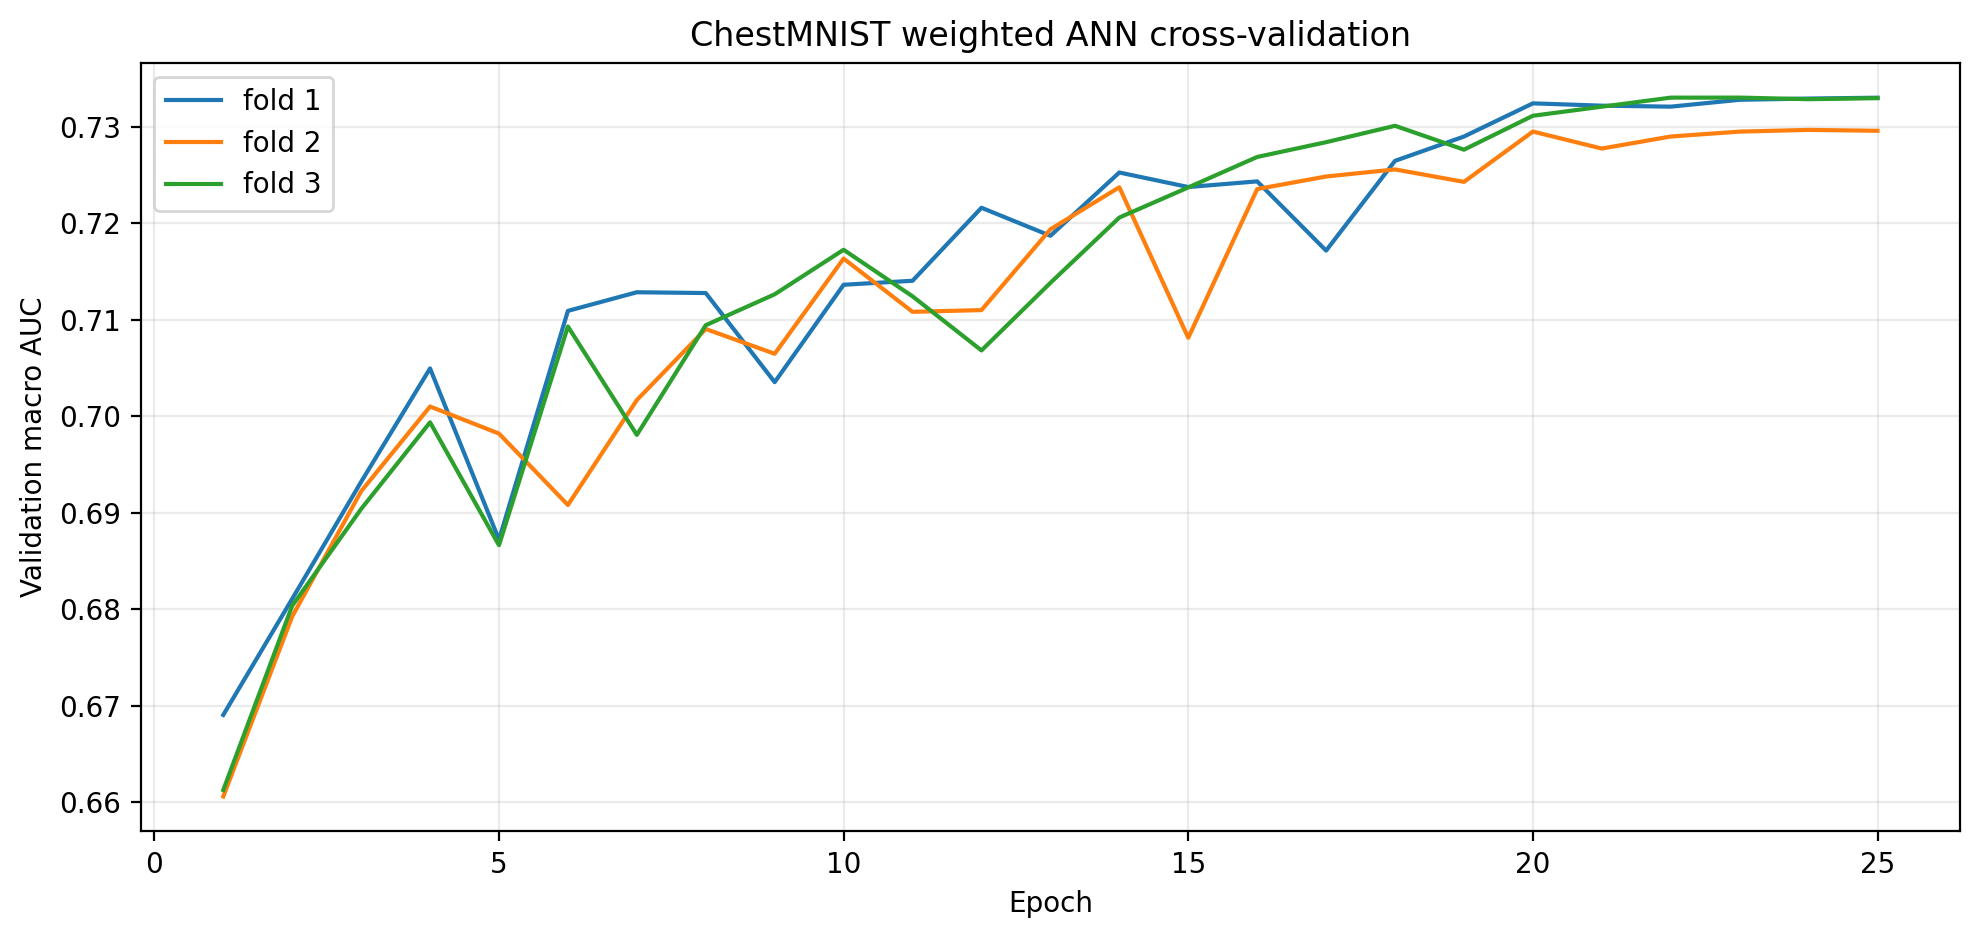
\includegraphics[width=0.95\textwidth]{figures/chestmnist-weighted-ann/cv_val_auc_curves.png}
  \caption{Đường cong validation macro AUC của 3 fold trong weighted CV ANN trên ChestMNIST.}
  \label{fig:chestmnist-cv-val-auc}
\end{figure}

\begin{figure}[H]
  \centering
  
\includegraphics[width=0.95\textwidth]{figures/chestmnist-weighted-ann/per_class_auc.png}
  \caption{AUC theo từng nhãn bệnh của weighted CV ANN ensemble trên ChestMNIST.}
  \label{fig:chestmnist-weighted-per-class-auc}
\end{figure}

\begin{figure}[H]
  \centering
  
\includegraphics[width=0.95\textwidth]{figures/chestmnist-weighted-ann/prevalence_vs_pred_rate.png}
  \caption{So sánh tỷ lệ dương thật và tỷ lệ dương dự đoán của weighted CV ANN ensemble trên ChestMNIST.}
  \label{fig:chestmnist-weighted-prevalence}
\end{figure}

Weighted CV ANN nâng \textit{test macro AUC} lên $0.7306$. Mặc dù \textit{test ACC} giảm xuống $0.7141$, đây lại là hướng cải thiện đúng với benchmark y sinh: mô hình bắt đầu chấp nhận dự đoán dương nhiều hơn, thay vì tối đa hóa số lượng nhãn âm đúng. Các đường cong validation AUC của ba fold cũng cho thấy chất lượng nội bộ giữa các lần chia không dao động quá lớn, tức là hướng cải tiến này không chỉ tăng trên một split cụ thể mà có độ ổn định tốt hơn baseline.

Sau bước này, insight rút ra là: thay đổi động lực học huấn luyện đã giúp ANN khai thác raw pixel tốt hơn, nhưng bản thân raw pixel vẫn chưa đủ giàu thông tin để đưa AUC lên sát các mốc benchmark mạnh hơn. Do đó, bước tiếp theo hợp lý là giữ lại weighted loss cùng protocol cross-validation, rồi bổ sung các handcrafted feature phù hợp với ảnh X-quang để đưa tín hiệu texture và cấu trúc vào ANN mà không cần chuyển sang CNN.

\subsection{Feature-fusion lite ANN}

Sau phương pháp 2, vấn đề còn lại không còn nằm chủ yếu ở loss hay protocol, mà ở bản thân biểu diễn đầu vào. Raw pixel giữ được cường độ sáng tại từng vị trí nhưng không mã hóa tường minh các tính chất texture và cấu trúc vốn quan trọng trong ảnh X-quang. Đây là lý do phương pháp 3 chuyển sang hướng \textit{feature fusion}: thay vì buộc ANN tự suy ra toàn bộ texture từ pixel thô, ta chủ động đưa vào những descriptor cổ điển vốn đã phù hợp với dữ liệu mức xám y sinh.

Biến thể cuối cùng của chương này là \textit{feature-fusion lite ANN}. Mỗi ảnh được biểu diễn bởi bốn nhóm đặc trưng: raw pixel, HOG, LBP histogram và intensity histogram. Mỗi nhóm giữ một vai trò khác nhau: raw pixel bảo toàn cường độ gốc; HOG mã hóa hướng gradient và biên cấu trúc; LBP histogram nhấn mạnh texture cục bộ; intensity histogram mô tả phân bố mức xám toàn ảnh. Cách ghép này xuất phát trực tiếp từ giả thuyết rằng ảnh X-quang cỡ nhỏ cần đồng thời cả thông tin biên lẫn texture để ANN phân biệt tốt hơn giữa các mẫu có tổn thương và mẫu bình thường. Các đặc trưng được nối lại thành một vector chung, rồi đưa qua MLP:
\[
\text{feature fusion} \rightarrow 1024 \rightarrow 512 \rightarrow 256 \rightarrow 14.
\]
Kiến trúc ẩn được giữ cùng khung $1024 \rightarrow 512 \rightarrow 256$ như phương pháp 2 để phép so sánh tập trung vào tác động của đầu vào mới thay vì bị nhiễu bởi việc đổi mạng quá nhiều. Việc không thay phần thân mạng giúp kết luận cuối cùng rõ ràng hơn: nếu AUC tăng, nguồn cải thiện chủ yếu phải đến từ chất lượng biểu diễn đầu vào và cơ chế tối ưu, chứ không phải do mạng đột ngột sâu hơn hay rộng hơn. Loss được đổi tiếp thành weighted focal BCE. Nếu \textit{pos\_weight} ở phương pháp 2 giải quyết vấn đề mất cân bằng lớp ở mức toàn cục, thì focal term của phương pháp 3 đi thêm một bước nữa: giảm trọng số của các mẫu quá dễ và tập trung gradient nhiều hơn vào các ca khó hoặc còn bị nhầm. Điều này đặc biệt phù hợp khi đầu vào đã giàu tín hiệu hơn, vì mô hình cần ưu tiên học các ranh giới quyết định khó thay vì tiếp tục tối ưu những mẫu âm dễ.

Protocol huấn luyện vẫn là \textit{3-fold cross-validation} trên split train chính thức và ensemble các fold ở bước test. Việc giữ nguyên protocol này là có chủ đích: nhờ đó, mọi cải thiện AUC ở phương pháp 3 có thể được quy về feature engineering và focal-weighted optimization, thay vì đến từ thay đổi cách đánh giá.

\begin{table}[H]
\centering
\caption{Kết quả của feature-fusion lite ANN ensemble trên ChestMNIST}
\label{tab:chestmnist-lite-results}
\begin{tabular}{l c}
\toprule
Chỉ số & Giá trị \\
\midrule
Feature set & raw + HOG + LBP histogram + intensity histogram \\
Kiến trúc mạng & feature fusion $\rightarrow 1024 \rightarrow 512 \rightarrow 256 \rightarrow 14$ \\
Số fold & 3 \\
Epoch mỗi fold & 40 \\
Optimizer & AdamW \\
Learning rate & 0.001 \\
Weight decay & 0.0001 \\
Loss & Weighted focal BCEWithLogits \\
Ensemble test macro AUC & 0.7424 \\
Ensemble test ACC & 0.7301 \\
Ensemble test macro F1 & 0.1667 \\
\bottomrule
\end{tabular}
\end{table}


\begin{figure}[H]
  \centering
  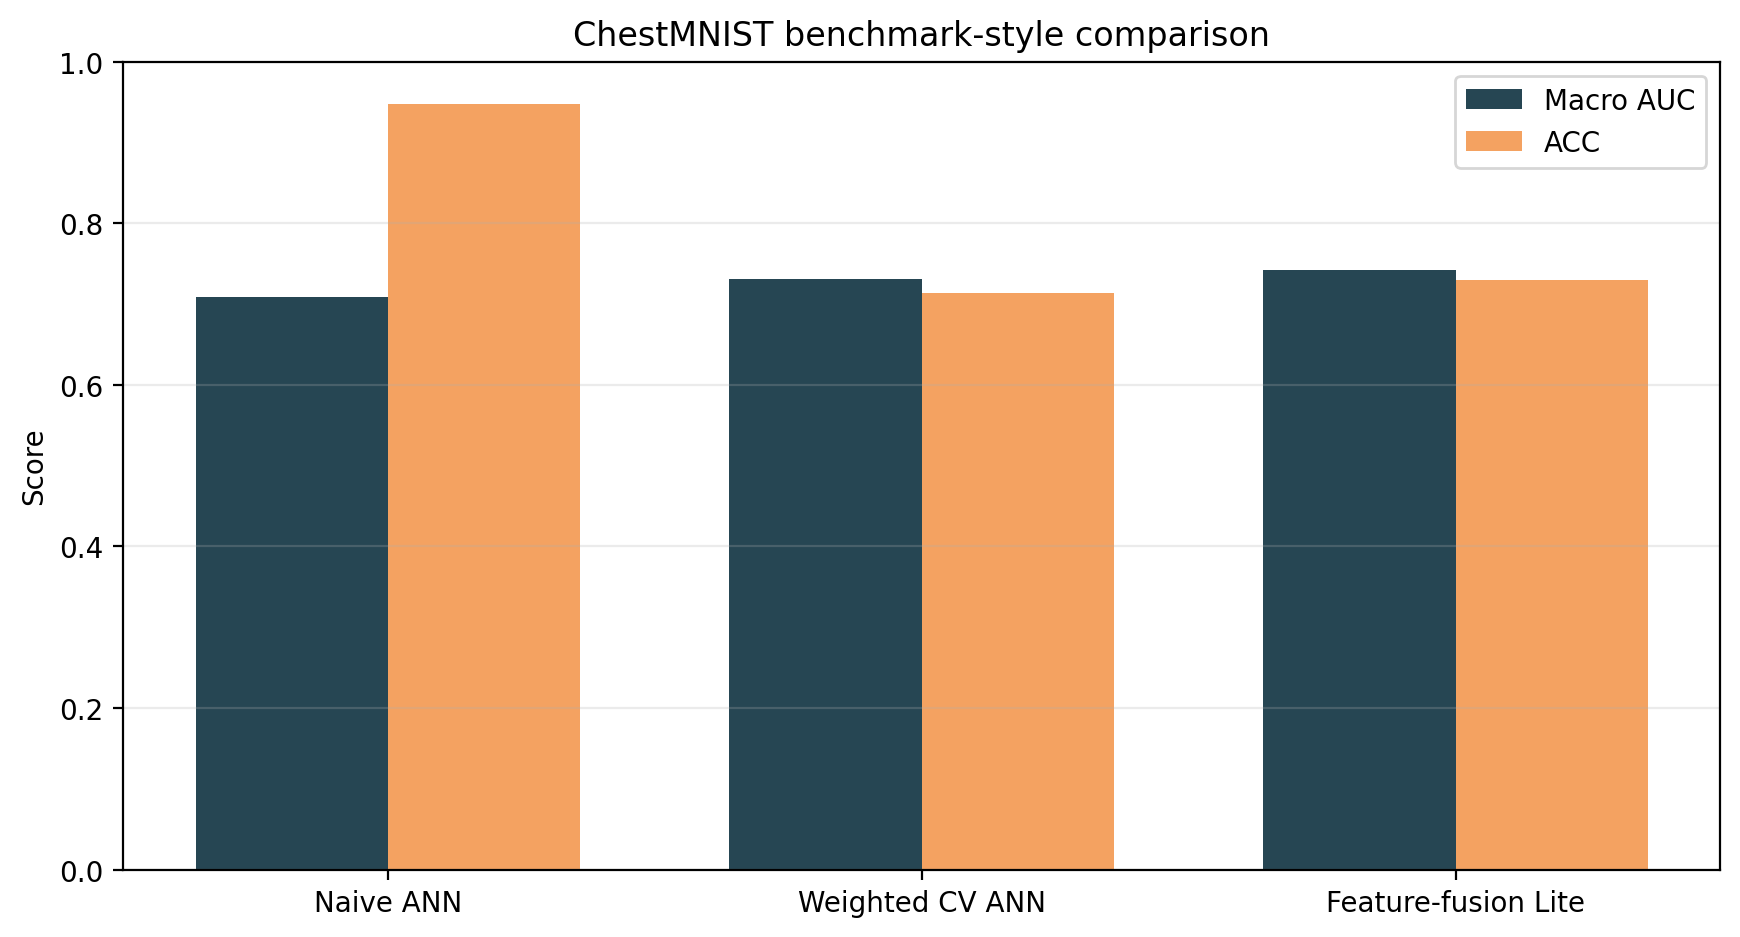
\includegraphics[width=0.95\textwidth]{figures/chestmnist-lite-ann/model_comparison.png}
  \caption{So sánh theo phong cách benchmark giữa ba cấu hình ANN trên ChestMNIST.}
  \label{fig:chestmnist-lite-model-comparison}
\end{figure}

\begin{figure}[H]
  \centering
  
\includegraphics[width=0.95\textwidth]{figures/chestmnist-lite-ann/per_class_auc.png}
  \caption{AUC theo từng nhãn bệnh của feature-fusion lite ANN trên ChestMNIST.}
  \label{fig:chestmnist-lite-per-class-auc}
\end{figure}

\begin{figure}[H]
  \centering
  
\includegraphics[width=0.95\textwidth]{figures/chestmnist-lite-ann/prevalence_vs_pred_rate.png}
  \caption{So sánh tỷ lệ dương thật và tỷ lệ dương dự đoán của feature-fusion lite ANN trên ChestMNIST.}
  \label{fig:chestmnist-lite-prevalence}
\end{figure}

Feature-fusion lite ANN đạt \textit{macro AUC} $0.7424$ và \textit{ACC} $0.7301$, trở thành cấu hình ANN tốt nhất hiện tại trên ChestMNIST trong repo. Mốc AUC này đã tiệm cận baseline AutoKeras trong benchmark chính thức của MedMNIST~\cite{medmnist_site}. Nói rõ hơn, AutoKeras là một công cụ AutoML xây trên Keras/TensorFlow, nên đây là một baseline mạnh và có uy tín, nhưng chưa phải mốc trần cao nhất của benchmark. Vì vậy, việc ANN thuần trong báo cáo đạt gần mức này có thể xem là kết quả tốt và đáng tin cậy, dù vẫn còn khoảng cách so với các baseline CNN như ResNet.

\section{Tổng hợp kết quả và nhận xét}

\begin{table}[H]
\centering
\caption{Kiến trúc ba biến thể ANN trên ChestMNIST}
\label{tab:chestmnist-ann-architecture-details}
\small
\begin{tabularx}{\textwidth}{>{\raggedright\arraybackslash}p{3.3cm} >{\raggedright\arraybackslash}p{3.1cm} >{\raggedright\arraybackslash}X >{\raggedright\arraybackslash}p{3.2cm}}
\toprule
Biến thể & Đầu vào & Kiến trúc & Thành phần chính \\
\midrule
Naive ANN & Raw $784$ & $784 \rightarrow 512 \rightarrow 256 \rightarrow 14$ & ReLU, BCEWithLogits \\
Weighted CV ANN & Raw $784$ & $784 \rightarrow 1024 \rightarrow 512 \rightarrow 256 \rightarrow 14$ & BN + Dropout + weighted BCE \\
Feature-fusion lite ANN & Raw + HOG + LBP + histogram & Feature fusion $\rightarrow 1024 \rightarrow 512 \rightarrow 256 \rightarrow 14$ & BN + Dropout + weighted focal BCE \\
\bottomrule
\end{tabularx}
\end{table}

\begin{table}[H]
\centering
\caption{Thông số huấn luyện của ba biến thể ANN trên ChestMNIST}
\label{tab:chestmnist-ann-hyperparameters}
\small
\begin{tabularx}{\textwidth}{>{\raggedright\arraybackslash}p{3.2cm} >{\raggedright\arraybackslash}p{3cm} >{\raggedright\arraybackslash}p{2.1cm} >{\raggedright\arraybackslash}X}
\toprule
Biến thể & Tối ưu hóa / loss & Batch/epoch & Thiết lập đặc trưng và đánh giá \\
\midrule
Naive ANN & Adam, BCEWithLogits & Theo notebook baseline / 45 & Raw pixel; dùng validation chính thức để theo dõi \\
Weighted CV ANN & AdamW, weighted BCE & 3 fold / 25 & Raw pixel; 3-fold multilabel stratified CV; ensemble fold \\
Feature-fusion lite ANN & AdamW, weighted focal BCE & 3 fold / 40 & Raw + HOG + LBP + histogram; 3-fold CV; ensemble fold \\
\bottomrule
\end{tabularx}
\end{table}

\begin{table}[H]
\centering
\caption{Logic chuyển từ một biến thể ANN sang biến thể kế tiếp trên ChestMNIST}
\label{tab:chestmnist-ann-iteration-logic}
\small
\begin{tabularx}{\textwidth}{>{\raggedright\arraybackslash}p{3.2cm} >{\raggedright\arraybackslash}X >{\raggedright\arraybackslash}X}
\toprule
Biến thể hiện tại & Điểm yếu quan sát được & Ý tưởng cho biến thể kế tiếp \\
\midrule
Naive ANN & AUC còn thấp; ACC cao nhưng chủ yếu do dự đoán âm nhiều & Thêm weighted loss và cross-validation để tăng khả năng tách ca bệnh \\
Weighted CV ANN & AUC tăng nhưng còn khoảng cách với benchmark mạnh hơn & Bổ sung handcrafted feature phù hợp với ảnh X-quang và dùng focal loss \\
\bottomrule
\end{tabularx}
\end{table}

\begin{table}[H]
\centering
\caption{So sánh hai cấu hình ANN trên ChestMNIST}
\label{tab:chestmnist-model-comparison}
\begin{tabular}{l c c c}
\toprule
Cấu hình & Test macro AUC & Test ACC & Ghi chú \\
\midrule
Naive ANN & 0.7088 & 0.9475 & BCE + $t=0.5$ \\
Weighted CV ANN & 0.7306 & 0.7141 & wBCE + CV + ensemble fold \\
Feature-fusion Lite ANN & 0.7424 & 0.7301 & feature fusion + focal + CV \\
\bottomrule
\end{tabular}
\end{table}


Các bảng tổng hợp cho thấy lộ trình cải tiến của Chương 3 khá nhất quán. Baseline naive cho ACC rất cao nhưng AUC còn thấp, vì mô hình hưởng lợi nhiều từ việc dự đoán âm. Weighted CV ANN sửa đúng điểm nghẽn này bằng cách thay đổi loss và protocol huấn luyện, từ đó nâng AUC lên rõ rệt. Feature-fusion lite ANN tiếp tục đẩy AUC lên $0.7424$ nhờ đưa thêm thông tin cấu trúc và texture phù hợp với ảnh X-quang vào đầu vào của ANN.

Kết luận cho Chương 3 có thể chốt bằng ba ý chính. Thứ nhất, baseline naive cho thấy raw pixel thuần vẫn học được tín hiệu phân biệt ở mức vừa phải theo AUC, nhưng chưa đủ để tạo ra một ANN mạnh trên dữ liệu y sinh đa nhãn. Thứ hai, bước cải tiến hiệu quả nhất không đến từ việc chỉ mở rộng MLP, mà từ việc thay đổi đúng động lực học huấn luyện bằng weighted loss, cross-validation và ensemble; chính tổ hợp này đã kéo macro AUC từ $0.7088$ lên $0.7306$. Thứ ba, cấu hình tốt nhất hiện tại là \textit{feature-fusion lite ANN} với macro AUC $0.7424$ và ACC $0.7301$, cho thấy việc đưa thêm HOG, LBP histogram và intensity histogram vào ANN là có giá trị thực nghiệm rõ ràng trên ChestMNIST. Vì vậy, insight quan trọng nhất của chương này là: với dữ liệu ảnh y sinh, hiệu quả của ANN phụ thuộc rất mạnh vào cách tổ chức đầu vào và cách thiết kế loss, chứ không thể chỉ kỳ vọng raw pixel phẳng tự mang đủ thông tin cho mô hình.
